\chapter{Scoping}

\section{Primo Project Scoping Meeting}

\subsection{Partecipanti}


\begin{center}
    \begin{tabular}{|l|l|}
        \hline
        \textbf{Ruolo}                   & \textbf{Partecipanti}              \\
        \hline
        Stakeholder                      & Rappresentanti della città di Roma \\
        \hline
        Project Manager                  & Alice Rossi                        \\
        \hline
        Architetti Software              & Giovanni Bianchi, Maria Verdi      \\
        \hline
        Sviluppatori Generici            & Marco Gialli, Laura Neri           \\
        \hline
        Esperti in IoT e Sensoristica    & Luca Azzurri                       \\
        \hline
        Esperti in Sicurezza Informatica & Andrea Blu                         \\
        \hline
        Facilitatore                     & Paolo Rossetti                     \\
        \hline
        Tecnografo                       & Giulia Rossini                     \\
        \hline
    \end{tabular}
\end{center}

\subsection{Agenda}

\begin{enumerate}
    \item \textbf{Introduzione}
          \begin{itemize}
              \item Presentazione del team e degli stakeholder presenti.
          \end{itemize}

    \item \textbf{Visione Generale del Progetto}
          \begin{itemize}
              \item Presentazione del progetto CityTwin e degli obiettivi.
          \end{itemize}

    \item \textbf{Discussione sui Requisiti Utente}
          \begin{itemize}
              \item Analisi e discussione dei requisiti utente identificati.
          \end{itemize}

    \item \textbf{Definizione dell'Ubiquitous Language}
          \begin{itemize}
              \item Creazione di un linguaggio comune per il team.
          \end{itemize}

    \item \textbf{Pianificazione dei Prossimi Passi}
          \begin{itemize}
              \item Discussione sulla struttura del progetto e definizione delle tappe successive.
          \end{itemize}

    \item \textbf{Domande e Risposte}
          \begin{itemize}
              \item Tempo dedicato a domande e chiarimenti.
          \end{itemize}

    \item \textbf{Chiusura del Meeting}
          \begin{itemize}
              \item Ringraziamenti e conferma dei prossimi passi.
          \end{itemize}
\end{enumerate}

\subsection{User Stories}

Nel corso del primo incontro di scoping, il team di progetto CityTwin ha identificato e definito le user stories chiave. Questa fase è stata fondamentale per ottenere una comprensione dettagliata delle esigenze degli utilizzatori finali e ha fornito una guida iniziale per lo sviluppo del sistema di digital twin.

\subsubsection{User Story 1: Visualizzazione dello Stato del Sistema tramite GUI}

\textbf{Come} utente interessato al monitoraggio del sistema CityTwin \\
\textbf{Voglio} accedere a una GUI (Control Panel) \\
\textbf{In modo da} visualizzare chiaramente lo stato attuale dei nodi Mainstay e Resource del sistema.

\textbf{Criteri di Accettazione:}
\begin{itemize}
    \item La GUI deve fornire un'interfaccia intuitiva e facile da comprendere.
    \item Lo stato di ciascun nodo (Mainstay e Resource) deve essere chiaramente indicato.
    \item L'utente deve essere in grado di distinguere facilmente i nodi online da quelli offline.
\end{itemize}

\subsubsection{User Story 2: Visualizzazione delle Risorse nella Città tramite GUI}

\textbf{Come} utente interessato alla localizzazione delle risorse nel sistema CityTwin \\
\textbf{Voglio} utilizzare la GUI \\
\textbf{In modo da} visualizzare la posizione delle risorse nella città, con indicazione del nome e dello stato (online/offline).

\textbf{Criteri di Accettazione:}
\begin{itemize}
    \item La mappa nella GUI deve mostrare chiaramente la posizione delle risorse.
    \item Ogni risorsa deve essere contrassegnata con il suo nome e stato di funzionamento.
    \item L'aggiornamento della posizione delle risorse deve essere in tempo reale.
\end{itemize}

\subsubsection{User Story 3: Monitoraggio Storico tramite GUI}

\textbf{Come} utente interessato all'analisi storica dei dati del sistema CityTwin \\
\textbf{Voglio} utilizzare la GUI \\
\textbf{In modo da} visualizzare un grafico che rappresenti il numero di nodi Mainstay e Resource online nel tempo, basato sui dati rilevati dal servizio di persistenza.

\textbf{Criteri di Accettazione:}
\begin{itemize}
    \item La GUI deve presentare un grafico temporale del numero di nodi online nel corso del tempo.
    \item L'asse delle ascisse deve rappresentare il tempo, mentre l'asse delle ordinate deve rappresentare il numero di nodi online.
    \item L'utente deve poter selezionare intervalli temporali specifici per l'analisi.
\end{itemize}

\subsection{Ubiquitous Language}

Durante lo stesso incontro, è stato stabilito un linguaggio comune (Ubiquitous Language) basato sulle specifiche del dominio del progetto CityTwin. Questo linguaggio è stato adottato da tutti i membri del team per garantire una comunicazione chiara e univoca.

\begin{itemize}
    \item \textbf{GUI (Control Panel):} Interfaccia grafica utente che fornisce una visione d'insieme dello stato del sistema CityTwin, consentendo agli utenti di monitorare i nodi Mainstay e Resource.

    \item \textbf{Nodo Mainstay:} Nodo fondamentale all'interno del sistema CityTwin che si occupa di coordinare le informazioni tra i nodi Resource, rilevare malfunzionamenti e salvare dati in modo persistente.

    \item \textbf{Nodo Resource:} Nodo che rappresenta sensori, attuatori o entità complesse all'interno del sistema CityTwin. La composizione di più nodi Resource forma un Digital Twin.

    \item \textbf{Digital Twin:} Rappresentazione digitale di entità fisiche all'interno della città, composta da uno o più nodi Resource.

\end{itemize}

\section{Secondo Project Scoping Meeting}

\subsection{Agenda}

\begin{enumerate}
    \item \textbf{Revisione dei Progressi}
          \begin{itemize}
              \item Breve riepilogo dei progressi dal primo meeting.
          \end{itemize}

    \item \textbf{Affinamento delle User Stories}
          \begin{itemize}
              \item Discussione e affinamento delle user stories identificate.
          \end{itemize}

    \item \textbf{Aggiornamento dell'Ubiquitous Language}
          \begin{itemize}
              \item Revisione e aggiornamento del linguaggio comune.
          \end{itemize}

    \item \textbf{Definizione delle Condition of Satisfaction}

    \item \textbf{Pianificazione delle Attività Future}
          \begin{itemize}
              \item Discussione sui passi successivi e assegnazione di compiti.
          \end{itemize}

    \item \textbf{Domande e Risposte}
          \begin{itemize}
              \item Tempo dedicato a domande e chiarimenti.
          \end{itemize}

    \item \textbf{Chiusura del Meeting}
          \begin{itemize}
              \item Ringraziamenti e conferma dei prossimi passi.
          \end{itemize}
\end{enumerate}

\subsection{User Stories}

In una sessione successiva, il team ha affinato ulteriormente le user stories. Questo passo è stato intrapreso per tenere conto di eventuali nuove informazioni emerse durante lo sviluppo iniziale del progetto, mirando a ottenere una comprensione più approfondita delle esigenze degli utenti.

\subsubsection{User Story 4: Monitoraggio dello Stato del fiume tramite GUI}

\textbf{Come} utente interessato al monitoraggio dello stato dei fiumi \\
\textbf{Voglio} utilizzare la GUI \\
\textbf{In modo da} visualizzare chiaramente lo stato attuale del River Monitor (Safe, Warned, Evacuating).

\textbf{Criteri di Accettazione:}
\begin{itemize}
    \item La GUI deve presentare lo stato corrente del River Monitor in modo evidente.
    \item Lo stato deve essere visivamente distintivo per una rapida interpretazione.
\end{itemize}

\subsubsection{User Story 5: Gestione dello Stato del River Monitor tramite GUI}

\textbf{Come} utente autorizzato alla gestione degli stati del River Monitor \\
\textbf{Voglio} utilizzare la GUI \\
\textbf{In modo da}  poter passare manualmente dallo stato di "Warned" a "Evacuating" e da "Evacuating" a "Safe".

\textbf{Criteri di Accettazione:}
\begin{itemize}
    \item La GUI deve fornire pulsanti chiaramente identificabili per passare tra gli stati.
    \item L'utente autorizzato deve poter effettuare la transizione di stato senza difficoltà.
\end{itemize}

\subsubsection{User Story 6: Aggiunta/Rimozione Nodi Resource in Tempo Reale}

\textbf{Come} amministratore del sistema CityTwin \\
\textbf{Voglio} avere la possibilità di aggiungere o rimuovere nuovi nodi Resource \\
\textbf{In modo da} adattare il sistema alle mutevoli esigenze delle smart city.

\textbf{Criteri di Accettazione:}
\begin{itemize}
    \item L'amministratore deve poter aggiungere nuovi nodi Resource senza interrompere il funzionamento del sistema.
    \item La rimozione di nodi Resource non deve causare problemi di integrità del sistema.
    \item Le modifiche devono essere effettive in tempo reale.
\end{itemize}

\subsection{Conditions of Satisfaction}

Derivate dalle richieste del committente emerse durante il nostro primo incontro, il team ha identificato le seguenti CoS per il progetto:

\begin{enumerate}
    \item \textbf{Vincoli di Budget:} Il completamento del progetto deve avvenire rispettando il budget preventivato per la sua esecuzione.

    \item \textbf{Vincoli di Tempo:} L'implementazione del progetto deve rispettare le tempistiche stabilite, garantendo una consegna puntuale.

    \item \textbf{Soddisfazione del Cliente:} Il prodotto deve non solo soddisfare le esigenze immediate del cliente, ma deve anche costituire una base solida per eventuali sviluppi futuri, assicurando la massima soddisfazione.

    \item \textbf{Rispetto del Piano di Qualità:} È essenziale conformarsi alle convenzioni adottate dalle diverse tecnologie utilizzate e rispettare gli standard concordati in tutte le fasi del progetto, garantendo un livello elevato di qualità.

    \item \textbf{Documentazione Completa dell'Architettura Software:} La documentazione deve essere chiara, completa e facilmente consultabile, pronta a fornire chiarimenti qualora necessario.

    \item \textbf{Modularità:} Il sistema deve essere realizzato in moduli separati, in modo da poter essere facilmente estendibile.

\end{enumerate}


\subsection{Ubiquitous Language}

Durante lo stesso incontro, il linguaggio comune è stato rivisto e aggiornato per riflettere meglio le dinamiche emergenti durante il processo di sviluppo. Questo assicura una comunicazione continua e chiara tra i membri del team.

\begin{itemize}
    \item \textbf{GUI (Control Panel):} Interfaccia grafica utente che fornisce una visione d'insieme dello stato del sistema CityTwin, consentendo agli utenti di monitorare i nodi Mainstay e Resource.

    \item \textbf{GUI (River Monitor):} Interfaccia grafica utente specifica per il monitoraggio dello stato del fiume, consentendo agli utenti di visualizzare informazioni cruciali come lo stato corrente e i livelli dell'acqua.

    \item \textbf{Nodo Mainstay:} Nodo fondamentale all'interno del sistema CityTwin che si occupa di coordinare le informazioni tra i nodi Resource, rilevare malfunzionamenti e salvare dati in modo persistente.

    \item \textbf{Nodo Resource:} Nodo che rappresenta sensori, attuatori o entità complesse all'interno del sistema CityTwin. La composizione di più nodi Resource forma un digital twin.

    \item \textbf{Digital Twin:} Rappresentazione digitale di entità fisiche all'interno della città, composta da uno o più nodi Resource.

    \item \textbf{River Monitor:} Parte del sistema CityTwin che si occupa del monitoraggio dello stato dei fiumi, incluso il livello dell'acqua e le transizioni tra gli stati Safe, Warned ed Evacuating.

\end{itemize}

\section{Terzo Project Scoping Meeting}

\subsection{Agenda}

\begin{enumerate}
    \item \textbf{Revisione dei Progressi}
          \begin{itemize}
              \item Breve riepilogo dei progressi dagli incontri precedenti.
          \end{itemize}

    \item \textbf{Validazione e Convalida delle User Stories}
          \begin{itemize}
              \item Riveduta e convalida delle user stories alla luce delle informazioni emerse.
          \end{itemize}

    \item \textbf{Consolidamento dell'Ubiquitous Language}
          \begin{itemize}
              \item Ulteriori raffinamenti e chiarimenti al linguaggio comune.
          \end{itemize}

    \item \textbf{Strutturazione della Requirement Breakdown Structure}
          \begin{itemize}
              \item Definizione della struttura gerarchica dei requisiti.
          \end{itemize}

    \item \textbf{Definizione del Project Overview Statement}

    \item \textbf{Domande e Risposte}
          \begin{itemize}
              \item Tempo dedicato a domande e chiarimenti.
          \end{itemize}

    \item \textbf{Chiusura del Meeting}
          \begin{itemize}
              \item Ringraziamenti e conferma dei prossimi passi.
          \end{itemize}
\end{enumerate}

\subsection{Requirement Breakdown Structure}

Il team ha proceduto con il definire la RBS (Requirement Breakdown Structure), in modo da ottenere una visione d'insieme delle funzionalità e delle caratteristiche del sistema. Questo diagramma è utile anche per il committente del progetto, in quanto fornisce una rappresentazione visiva dei requisiti e delle relazioni tra di essi.

\begin{figure}[H]
    \centering
    \caption{Requirement Breakdown Structure.}
    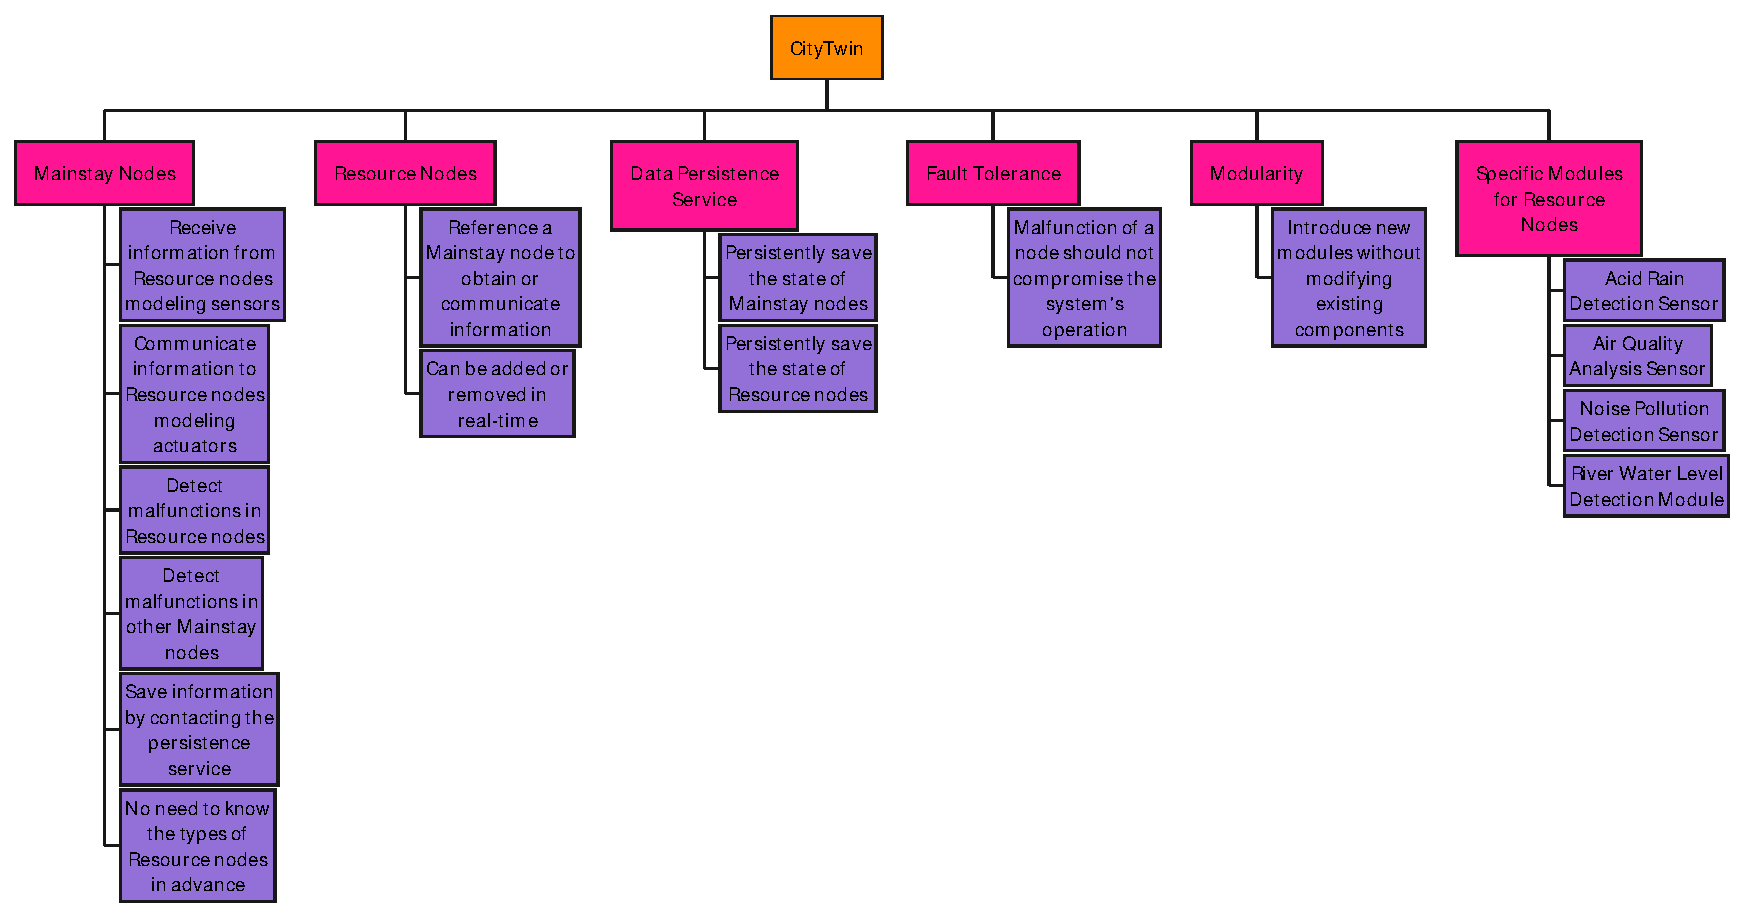
\includegraphics[height=.8\textwidth, angle=90]{figures/RBS.pdf}
    \label{fig:rbs}
\end{figure}

\subsection{Project Overview Statement}

\subsubsection{Problema/Opportunità}

Il progetto CityTwin si propone di affrontare la complessità della gestione urbana attraverso una piattaforma innovativa di monitoraggio delle smart city.

\subsubsection{Goal del Progetto}

L'obiettivo principale di CityTwin è fornire una piattaforma completa e flessibile per il monitoraggio delle smart city, consentendo una gestione efficiente delle risorse urbane e migliorando l'esperienza complessiva degli abitanti.

\subsubsection{Obiettivi del Progetto}

\begin{enumerate}
    \item \textbf{Creazione della Piattaforma:} Sviluppare una piattaforma di monitoraggio, integrando moduli specifici per la gestione avanzata di sensori e attuatori.

    \item \textbf{Implementazione di Nodi Mainstay e Resource:} Realizzare nodi Mainstay per la comunicazione efficace e nodi Resource per rappresentare entità urbane, garantendo una gestione dinamica in tempo reale.

    \item \textbf{Integrazione di Moduli:} Integrare nuovi moduli, come sensori per la qualità dell'aria e monitoraggio dello stato del fiume, senza compromettere la stabilità del sistema.
\end{enumerate}

\subsubsection{Criteri di Successo}

Il successo del progetto CityTwin sarà valutato in base ai seguenti criteri quantitativi:

\begin{enumerate}
    \item \textbf{Funzionalità Operative:} La piattaforma deve consentire la visualizzazione accurata dello stato della città digitale e il monitoraggio in tempo reale delle risorse.

    \item \textbf{Risposta Tempestiva:} Il tempo di risposta del sistema deve rispettare i limiti prestabiliti, garantendo un'esperienza utente efficiente.

    \item \textbf{Affidabilità e Ridondanza:} La ridondanza implementata deve mantenere la continuità operativa anche in caso di guasti hardware o malfunzionamenti.
\end{enumerate}

\subsubsection{Assunzioni, Rischi e Ostacoli}

\paragraph{Assunzioni}

\begin{enumerate}
    \item Si assume una collaborazione attiva tra i membri del team e gli stakeholder per garantire una comprensione condivisa degli obiettivi.

    \item Si presuppone la disponibilità delle risorse umane e tecnologiche necessarie per lo sviluppo e l'implementazione del progetto.
\end{enumerate}

\paragraph{Rischi e Ostacoli}

\begin{enumerate}
    \item Ci sono rischi legati alla disponibilità e affidabilità dei dati raccolti dai nodi Resource, che potrebbero essere influenzati da fattori come guasti hardware o interferenze ambientali.
    \item La sincronizzazione continua dei nodi Mainstay rappresenta un ostacolo tecnico significativo, poiché richiede una rete robusta e una gestione accurata degli aggiornamenti software.
    \item Potenziali rischi per la privacy dei dati, servono robuste misure di cybersecurity per proteggere informazioni sensibili.
    \item L'implementazione potrebbe affrontare ostacoli legati all'interoperabilità di vari sistemi e dispositivi.
\end{enumerate}

\subsection{Project Management Life Cycle}

La decisione di adottare una metodologia Agile all'interno del Project Management Life Cycle (PMLC) per il progetto CityTwin è stata basata su una serie di considerazioni strategiche e operazionali. L'approccio Agile è stato scelto per affrontare specifiche esigenze del progetto e per massimizzare l'efficienza nello sviluppo della piattaforma di monitoraggio delle smart city.

\subsubsection{Motivazioni della Scelta}

\begin{enumerate}
    \item \textbf{Adattabilità alle Variazioni dei Requisiti:} Nel contesto delle smart city, i requisiti possono evolvere rapidamente a causa dei cambiamenti nell'ambiente urbano o delle nuove esigenze degli utenti. L'Agile, con i suoi principi di risposta al cambiamento, consente al team di adattarsi in modo flessibile a nuovi requisiti senza dover riprogettare l'intero processo.

    \item \textbf{Coinvolgimento Continuo degli Stakeholder:} La metodologia Agile promuove una comunicazione costante e una collaborazione attiva con gli stakeholder.

    \item \textbf{Consegne Incrementali e Rapide:} La natura iterativa dello sviluppo Agile consente la realizzazione di funzionalità incrementali e il rilascio tempestivo di prodotti intermedi. Questo approccio è particolarmente vantaggioso per il progetto CityTwin, in cui è possibile fornire valore ai clienti attraverso funzionalità parziali già durante il processo di sviluppo.

    \item \textbf{Gestione Efficace dei Rischi:} La metodologia Agile facilita l'identificazione e la gestione tempestiva dei rischi. Attraverso la pianificazione di sprint e la regolare revisione dei risultati ottenuti, il team può rapidamente adattarsi a eventuali sfide o cambiamenti nelle condizioni di progetto.

    \item \textbf{Focus sulla Qualità e Test Continuo:} La pratica dell'Agile di integrare il controllo della qualità e i test durante tutto il ciclo di sviluppo favorisce la creazione di un prodotto finale più robusto e di alta qualità. Questo è particolarmente rilevante per il progetto CityTwin, dove la precisione e l'affidabilità delle informazioni sono essenziali per il corretto funzionamento del sistema.
\end{enumerate}

\subsubsection{Implementazione Pratica dell'Agile nel PMLC}

\begin{enumerate}
    \item \textbf{Sprint Planning Meetings:} Il lavoro è organizzato in sprint, ciascuno con una durata definita. Durante le riunioni di pianificazione degli sprint, il team identifica le attività prioritarie da completare durante il prossimo ciclo di sviluppo.

    \item \textbf{Daily Stand-Ups:} Breve riunione quotidiana in cui i membri del team condividono aggiornamenti sul proprio lavoro, identificano ostacoli e pianificano le azioni correttive. Questa pratica promuove la trasparenza e la collaborazione continua.

    \item \textbf{Backlog di Prodotto Dinamico:} Il backlog del prodotto, contenente tutte le funzionalità pianificate, è soggetto a cambiamenti durante il progetto. Nuovi requisiti o modifiche possono essere aggiunti in qualsiasi momento, garantendo una risposta rapida alle esigenze emergenti.

    \item \textbf{Continuous Integration e Continuous Deployment (CI/CD):} L'uso di pratiche CI/CD consente al team di integrare costantemente il codice e di rilasciare nuove versioni del software in modo rapido e affidabile, garantendo un flusso di lavoro continuo.

    \item \textbf{Retrospective Meetings:} Alla fine di ogni sprint, il team partecipa a riunioni retrospective per valutare ciò che è stato realizzato, identificare miglioramenti possibili nel processo e pianificare regolazioni per gli sprint successivi.

    \item \textbf{Flessibilità nell'Implementazione dei Moduli:} L'Agile offre la flessibilità necessaria per introdurre nuovi moduli nel sistema senza dover attendere la conclusione del ciclo di sviluppo complessivo. Questo è particolarmente utile per il progetto CityTwin, dove l'evoluzione delle tecnologie o l'emergere di nuove esigenze richiede una risposta immediata.
\end{enumerate}
